\section{Введение}\label{ux432ux432ux435ux434ux435ux43dux438ux435}

В рамках курса было необходимо разработать приложение, позволяющее
продемонстировать применение основных принципов проектирования
программного обеспечения. В частности, в приложении необходимо было
выделить следующие компоненты:

\begin{itemize}
\tightlist
\item
  Слой бизнес-логики
\item
  Слой хранения данных
\item
  Слой представления
\end{itemize}

Было решено разработать информационную систему для научного журнала.

\section{Роли}\label{ux440ux43eux43bux438}

В проекте выделено 3 роли: исследователь, редакция и рецензент:

\begin{enumerate}
\def\labelenumi{\arabic{enumi}.}
\tightlist
\item
  Исследователь
\end{enumerate}

\begin{itemize}
\tightlist
\item
  Разрабатывает научную тему
\item
  Пишет статью по ней
\item
  Принимает замечания по ней
\item
  Цель: Чтобы его статья была опубликована в журнале
\end{itemize}

\begin{enumerate}
\def\labelenumi{\arabic{enumi}.}
\setcounter{enumi}{1}
\tightlist
\item
  Рецензент
\end{enumerate}

\begin{itemize}
\tightlist
\item
  Выбирается редакцией
\item
  Получает статьи для просмотра
\item
  Дает оценку статье (стоит ли принимать для публикации)
\item
  Высказывает замечания, возникшие при прочтении статьи
\item
  Цель: Выбрать подходящие статьи
\end{itemize}

\begin{enumerate}
\def\labelenumi{\arabic{enumi}.}
\setcounter{enumi}{2}
\tightlist
\item
  Редакция
\end{enumerate}

\begin{itemize}
\tightlist
\item
  Принимает статьи
\item
  Устанавливает правила принятия статей
\item
  Подбирает рецензентов
\item
  Связывает рецензентов и авторов
\item
  Корректирует статьи, если необходимо
\item
  Издает журнал с помощью типографии
\item
  Цель: Принять качественные статьи, заработать на продаже журналов
\end{itemize}

\section{Варианты
использования}\label{ux432ux430ux440ux438ux430ux43dux442ux44b-ux438ux441ux43fux43eux43bux44cux437ux43eux432ux430ux43dux438ux44f}

\subsection{Написание
статьи}\label{ux43dux430ux43fux438ux441ux430ux43dux438ux435-ux441ux442ux430ux442ux44cux438}

\begin{enumerate}
\def\labelenumi{\arabic{enumi}.}
\tightlist
\item
  \textbf{Исследователь} выбирает \textbf{тему} и при поддержке научного
  руководителя проводит исследования
\item
  По результататам исследований автор при поддержке соавторов пишет
  \textbf{научную статью}
\item
  Автор выбирает \textbf{журнал} для публикации
\item
  Автор получает от редакторов журнала \textbf{правила оформления}
\item
  Автор редактирует статью в соответствии с правилами
\end{enumerate}

\begin{itemize}
\tightlist
\item
  Альтернатива: Редакция журнала сама готова привести
  \textbf{форматирование} к требуемому виду
\end{itemize}

\subsection{Подача}\label{ux43fux43eux434ux430ux447ux430}

\begin{enumerate}
\def\labelenumi{\arabic{enumi}.}
\tightlist
\item
  Автор отправляет статью в \textbf{систему подачи статей}
\item
  \textbf{Редакция} просматривает статью
\item
  Статья передается на рецензирование
\end{enumerate}

\begin{itemize}
\tightlist
\item
  Альтернатива: Редакция отказывает в приеме статьи и отправляет
  исследователю \textbf{список замечаний}, чтобы он их исправил
\item
  Альтернатива: Редакция отказывает в приеме и рекомендует автору
  отправить статью в \textbf{другой журнал}
\end{itemize}

\subsection{Рецензирование}\label{ux440ux435ux446ux435ux43dux437ux438ux440ux43eux432ux430ux43dux438ux435}

\begin{enumerate}
\def\labelenumi{\arabic{enumi}.}
\tightlist
\item
  Редакторы подбирают \textbf{рецензентов} и отправляют им статью
\item
  Рецензенты читают статью и составляют \textbf{отчет} по ней,
  содержащий \textbf{вопросы}, \textbf{замечания} и \textbf{общую оценку
  статьи}
\item
  Редакторы пересылают вопросы и замечания исследователю
\item
  В соответствии с оценкой редакция принимает \textbf{решение} о
  публикации
\end{enumerate}

\begin{itemize}
\tightlist
\item
  Альтернатива: Редакция отказывает в публикации, статья дорабатывается
  и передается либо на этап рецензирования, либо на этап подачи, либо в
  другой журнал
\end{itemize}

\subsection{Подготовка и
публикация}\label{ux43fux43eux434ux433ux43eux442ux43eux432ux43aux430-ux438-ux43fux443ux431ux43bux438ux43aux430ux446ux438ux44f}

\begin{enumerate}
\def\labelenumi{\arabic{enumi}.}
\tightlist
\item
  Редакция адаптирует статью под \textbf{макет журнала}
\item
  Редакция исправляет \textbf{ошибки правописания}
\item
  Статья помещается в \textbf{пул публикаций}, которые будут
  опубликованы в следующем \textbf{выпуске} журнала
\end{enumerate}

\begin{itemize}
\tightlist
\item
  Альтернатива: В дополнение к журналу, статья может быть
  \textbf{опубликована онлайн} индивидуально. Это происходит сразу же,
  без ожидания следующего выпуска журнала
\end{itemize}

\begin{enumerate}
\def\labelenumi{\arabic{enumi}.}
\setcounter{enumi}{3}
\tightlist
\item
  Журнал из статей отправляется в \textbf{типографию}
\end{enumerate}

\begin{itemize}
\tightlist
\item
  Альтернатива: В дополнение к печатному варианту, журнал может быть
  опубликован в цифровом варианте
\end{itemize}

\section{Диаграмма вариантов
использования}\label{ux434ux438ux430ux433ux440ux430ux43cux43cux430-ux432ux430ux440ux438ux430ux43dux442ux43eux432-ux438ux441ux43fux43eux43bux44cux437ux43eux432ux430ux43dux438ux44f}

\begin{figure}[htbp]
\centering
\includegraphics{https://raw.githubusercontent.com/h31/SoftwareArchitecture/master/UseCases.png}
\caption{Диаграмма вариантов использования}
\end{figure}

\section{Диаграмма
классов}\label{ux434ux438ux430ux433ux440ux430ux43cux43cux430-ux43aux43bux430ux441ux441ux43eux432}

\begin{figure}[htbp]
\centering
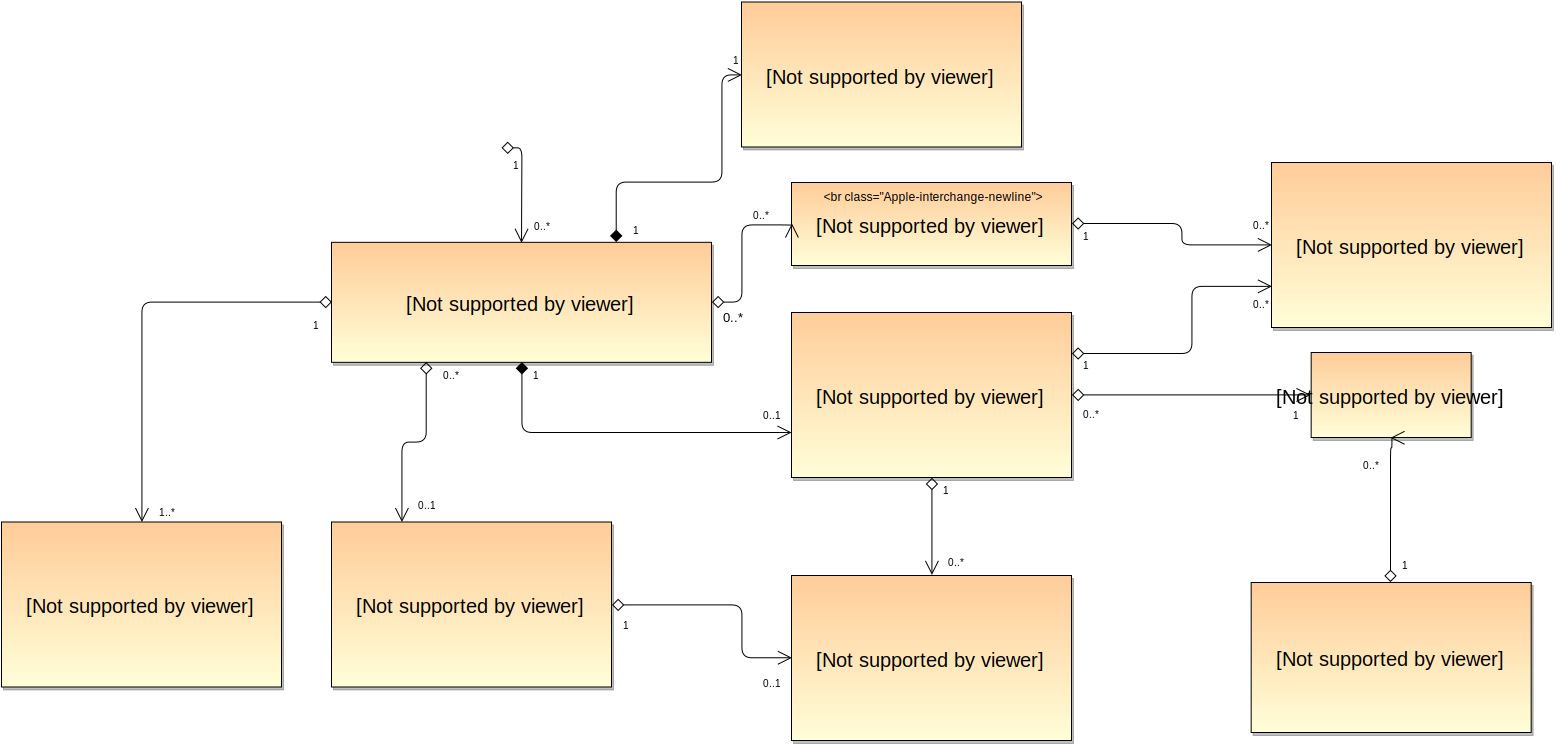
\includegraphics{https://raw.githubusercontent.com/h31/SoftwareArchitecture/master/ClassDiagram.png}
\caption{Диаграмма классов}
\end{figure}

\section{Диаграмма
последовательностей}\label{ux434ux438ux430ux433ux440ux430ux43cux43cux430-ux43fux43eux441ux43bux435ux434ux43eux432ux430ux442ux435ux43bux44cux43dux43eux441ux442ux435ux439}

\subsection{Написание статьи и отправка в
журнал}\label{ux43dux430ux43fux438ux441ux430ux43dux438ux435-ux441ux442ux430ux442ux44cux438-ux438-ux43eux442ux43fux440ux430ux432ux43aux430-ux432-ux436ux443ux440ux43dux430ux43b}

\begin{figure}[htbp]
\centering
\includegraphics{https://raw.githubusercontent.com/h31/SoftwareArchitecture/master/Seq1.png}
\caption{Seq1}
\end{figure}

\subsection{Рецензирование}\label{ux440ux435ux446ux435ux43dux437ux438ux440ux43eux432ux430ux43dux438ux435-1}

\begin{figure}[htbp]
\centering
\includegraphics{https://raw.githubusercontent.com/h31/SoftwareArchitecture/master/Seq2.png}
\caption{Seq2}
\end{figure}

\section{Проектирование слоя
бизнес-логики}\label{ux43fux440ux43eux435ux43aux442ux438ux440ux43eux432ux430ux43dux438ux435-ux441ux43bux43eux44f-ux431ux438ux437ux43dux435ux441-ux43bux43eux433ux438ux43aux438}

В качестве архитектурного шаблона был выбран шаблон ``Модель предметной
области''. В связи с этим, были выделены сущности предметной области и
для каждой из сущностей было решено создать отдельный класс, описывающий
данную сущность. Написанные классы расположены в пакете objects.

\section{Реализация слоя
бизнес-логики}\label{ux440ux435ux430ux43bux438ux437ux430ux446ux438ux44f-ux441ux43bux43eux44f-ux431ux438ux437ux43dux435ux441-ux43bux43eux433ux438ux43aux438}

Для классов слоя бизнес-логики был создан пакет services.

Основной класс бизнес-логики - SubmissionUpdate. Он содержит методы,
помогающие ``продвигать'' статью по цепочке
редакция-рецензент-издательство.

\section{Проектирование слоя хранения
данных}\label{ux43fux440ux43eux435ux43aux442ux438ux440ux43eux432ux430ux43dux438ux435-ux441ux43bux43eux44f-ux445ux440ux430ux43dux435ux43dux438ux44f-ux434ux430ux43dux43dux44bux445}

Для слоя хранения был выбран паттерн ``Преобразователь данных'' (Data
Mapper), ввиду того, что он хорошо подходит под паттерн ``Модель
предметной области''. Все классы, связанные с хранением данных,
содержатся в пакете storage. Имеются две реализации слоя хранения: на
основе коллекций Java (в пакете storage.java) и на основе РСУБД (в
пакете storage.mappers). Для абстрагирования сервисов от конкретного
слоя использовался набор интерфейсов, соответствующих названию сущности
(например, PaperStorage).

\section{Реализация слоя хранения
данных}\label{ux440ux435ux430ux43bux438ux437ux430ux446ux438ux44f-ux441ux43bux43eux44f-ux445ux440ux430ux43dux435ux43dux438ux44f-ux434ux430ux43dux43dux44bux445}

В качестве СУБД было решено использовать PostgreSQL по причине того, что
она уже была установлена и настроена на используемом компьютере. В
начале работы над проектом использовалась HyperSQL, однако из-за малой
функциональности пришлось отказаться от неё.

Для удобства, в качестве первичного ключа использовались UUID. Генерация
ключей происходила на стороне приложения.

\section{Проектирование тестового
набора}\label{ux43fux440ux43eux435ux43aux442ux438ux440ux43eux432ux430ux43dux438ux435-ux442ux435ux441ux442ux43eux432ux43eux433ux43e-ux43dux430ux431ux43eux440ux430}

Для тестирования использовался фреймворк JUnit 4. Тесты по своей сути
повторяют варианты использования.

\section{Проектирование слоя
представления}\label{ux43fux440ux43eux435ux43aux442ux438ux440ux43eux432ux430ux43dux438ux435-ux441ux43bux43eux44f-ux43fux440ux435ux434ux441ux442ux430ux432ux43bux435ux43dux438ux44f}

Было решено разработать Web-интерфейс. В качестве Web-сервера
использовался Spark (на основе Jetty 9.3). Для генерации страниц на
стороне сервера использовалась библиотека Thymeleaf. Весь код, связанный
с интерфейсом пользователя, находится в пакете UI. Основной класс -
WebUI.

В проекте имеются 4 HTML-страницы - по одной для каждой роли, плюс index
для навигации.

Ниже приведены примеры страниц.

\includegraphics{https://raw.githubusercontent.com/h31/SoftwareArchitecture/master/ResearcherUI.png}
\includegraphics{https://raw.githubusercontent.com/h31/SoftwareArchitecture/master/EditorUI.png}
\includegraphics{https://raw.githubusercontent.com/h31/SoftwareArchitecture/master/ReviewerUI.png}

\subsection{Реализация интеграции со сторонними
сервисами}\label{ux440ux435ux430ux43bux438ux437ux430ux446ux438ux44f-ux438ux43dux442ux435ux433ux440ux430ux446ux438ux438-ux441ux43e-ux441ux442ux43eux440ux43eux43dux43dux438ux43cux438-ux441ux435ux440ux432ux438ux441ux430ux43cux438}

Для реализации сервиса, отвечающего за поиск похожих статей, был создан
отдельный класс SimilarPapers.

В качестве источника данных использовался arXiv API.
\href{http://export.arxiv.org/api/query?search_query=cats\&start=0\&max_results=5}{Пример
запроса к API}.

Для REST-интерфейса со стороны приложения была выбрана функциональность
выгрузки готовых к печати статей в журнал. Пример выдачи в формате JSON:

\begin{verbatim}
[ {
  "state" : "IN_POOL",
  "paper" : {
    "id" : "a6230614-e8c2-4651-8f78-8285e8662626",
    "title" : "Code Uglify",
    "authors" : [ {
      "name" : "Peter",
      "university" : "MIT"
    } ],
    "keywords" : [ ],
    "abstractTxt" : "Abstract",
    "content" : "Text"
  },
  "reviewerRemark" : {
    "reviewer" : {
      "name" : "Rodrigo",
      "university" : "CMU",
      "id" : "0ae4f284-c5e4-4a41-bd4d-04af51974b36"
    },
    "mark" : "ACCEPT",
    "text" : "OK",
    "id" : "d5f7ad31-6bc9-44aa-a65a-f72d114bd068"
  },
  "editorialRemark" : {
    "id" : "4ac37a8a-f82a-4f67-ae9d-24e727e1aa4a",
    "decision" : "ACCEPT",
    "remark" : ""
  },
  "date" : 1465159744865
} ]
\end{verbatim}

Пример выдачи в формате XML:

\begin{verbatim}

<ArrayList>
  <item>
    <state>IN_POOL</state>
    <paper>
      <id>a6230614-e8c2-4651-8f78-8285e8662626</id>
      <title>Code Uglify</title>
      <authors>
        <authors>
          <name>Peter</name>
          <university>MIT</university>
        </authors>
      </authors>
      <keywords/>
      <abstractTxt>Abstract</abstractTxt>
      <content>Text</content>
    </paper>
    <reviewerRemark>
      <reviewer>
        <name>Rodrigo</name>
        <university>CMU</university>
        <id>0ae4f284-c5e4-4a41-bd4d-04af51974b36</id>
      </reviewer>
      <mark>ACCEPT</mark>
      <text>OK</text>
      <id>d5f7ad31-6bc9-44aa-a65a-f72d114bd068</id>
    </reviewerRemark>
    <editorialRemark>
      <id>4ac37a8a-f82a-4f67-ae9d-24e727e1aa4a</id>
      <decision>ACCEPT</decision>
      <remark></remark>
    </editorialRemark>
    <date>1465159744865</date>
  </item>
</ArrayList>
\end{verbatim}

\section{Заключение}\label{ux437ux430ux43aux43bux44eux447ux435ux43dux438ux435}

В рамках данного курса были изучены принципы разработки архитектуры
программного обеспечения, а так же, следуя этим принципам, было
разработано приложение. в приложении было создано три слоя:

\begin{itemize}
\tightlist
\item
  Слой бизнес-логики
\item
  Слой хранения данных
\item
  Слой представления
\end{itemize}
